\documentclass[epsfig,10pt,fullpage]{article}

\newcommand{\LabNum}{1}
\newcommand{\CommonDocsPath}{../../common/docs}
\input{\CommonDocsPath/preamble.tex}

\begin{document}

\centerline{\huge OPAE}
~\\
\centerline{\huge Laboratory Exercise \LabNum}
~\\
\centerline{\large Designing and Implementing an Intel AFU}
~\\

\noindent
This is an introductory exercise about heterogeneous computing using Intel technology.
Figure~\ref{fig:hetero} depicts a computer that includes both an 
Intel\textsuperscript{\textregistered} processor and a {\it Field-Programmable Gate Array}
(FPGA). The FPGA is a programmable logic device, which can be configured to implement
whatever hardware circuit is needed for a particular application.  
In the computer, the main circuit board that
houses the processor is connected to the FPGA board via a {\it PCI express} (PCIe) port.
In this introductory exercise we will show how to utilize the system in 
Figure~\ref{fig:hetero} as a {\it heterogeneous} 
computer in which both the processor and FPGA are used together to implement a computation.

~\\
\noindent
For the development of heterogeneous computing applications Intel
provides a set of tools called the {\it Intel Acceleration Stack}. It includes 
features for the development of both hardware and software components, as well as various 
mechanisms for connecting these components together. 
To gain access to the {\it Intel Acceleration Stack} we will make use of a cloud-based 
computing service called the Intel FPGA DevCloud\textsuperscript{\textregistered}.
The DevCloud offers server-class computers that contain both a high-end Intel processor
and an Intel Arria\textsuperscript{\textregistered} 10 FPGA.

\begin{figure}[b!]
   \begin{center}
       \includegraphics[scale=1.0]{figures/heterogeneous.pdf}
   \end{center}
   \caption{A heterogeneous computer.}
	\label{fig:hetero}
\end{figure}

~\\
\noindent
In various parts of this exercise you will need to execute commands within the DevCloud 
computing environment. This means that you are expected to obtain a {\it user account} on this
cloud service and to be familiar with its use. Instructions for obtaining access to the Intel
FPGA DevCloud, as well as an introduction to this computing environment, can be found
in the tutorial {\it Introduction to the Intel FPGA DevCloud}. This tutorial 
is provided by the Intel FPGA Academic Program and is available for download along with 
this laboratory exercise. 

~\\
\noindent
In a heterogeneous computing application, Intel refers to the part of the system
implemented in an FPGA as an {\it Accelerator Functional Unit} (AFU). In this exercise you
will design an AFU that provides a hardware component which is used to solve part of a
computation.  To complete the design of this AFU you will need 
to have a good grasp of the Verilog hardware description language 
(including some System Verilog extensions), which is used in the design of the 
AFU hardware, and the C programming language, which is used to write software programs 
for the processor that make use of the AFU. A good working knowledge of Linux is also 
desirable, as this is the operating system deployed on the Intel FPGA DevCloud. 

~\\
\noindent
This exercise is organized into the following stages:

\begin{enumerate}
\item Design a hardware component that will form the main part of an AFU. At this stage
the component will be just a ``normal'' hardware {\it module} specified in Verilog code. 
This module should be developed using a computer of your own choice (the DevCloud 
is not needed at this stage). We expect that you will compile and test your Verilog code 
on your own computer using a simulation tool with a Verilog {\it testbench}.
\item Augment the hardware component described above to create an AFU. This step involves 
adding specific ports and hardware registers that are required in the Verilog code for an AFU.
The AFU's registers will be memory-mapped to a specific part of the processor's address
space. To compile the AFU we will make use of the hardware development tools that are provided on 
the DevCloud.
\item Design software applications that utilize the AFU to perform computations
along with a processor. The software code will be compiled using the software 
development tools on the DevCloud.
\end{enumerate}

\section*{Part I}
Figure~\ref{fig:block} provides a high-level block diagram of an AFU connected to a 
processor via a {\it PCI Express} (PCIe) port.  The
part of the system implemented in the FPGA, highlighted in a blue color, is called the
{\it FPGA Interface Manager} (FIM). The FIM comprises two main components: the {\it FPGA
Interface Unit} (FIU) and the {\it AFU}. The purpose of the FIU is to act as a bridge
between the PCIe interface and the AFU. As indicated in the figure the FIU is connected to the
AFU via a {\it Protocol Port}. This port can implement a number of
communication protocols based on the AFU designer's preference. For this exercise we will
use the {\it Core Cache Interface} protocol\textsuperscript{\textregistered} (CCI-P), 
which is discussed in Part II. 

~\\
\begin{figure}[H]
   \begin{center}
       \includegraphics[scale=1.0]{figures/block.pdf}
   \end{center}
   \caption{A block diagram.}
	\label{fig:block}
\end{figure}

\newpage
\noindent
The AFU in Figure~\ref{fig:block} includes logic circuitry that facilitates access via
the protocol (CCI-P) port to some {\it registers}.
This circuitry provides address decoding that allows the processor to read/write 
AFU registers using memory-mapped I/O. Some of these registers have dedicated purposes 
that are required to be compatible with the Intel Acceleration Stack. Other registers are part
of the {\it Application Logic} in the AFU, which is the part of the AFU that is used to
perform computations along with the processor.

~\\
\noindent
The purpose of the AFU in this exercise is to provide a hardware module that generates 
{\it random} integers. The processor can configure the AFU so that it produces integers 
within a desired range, or to affect the sequence of values that are generated. Whenever
it is required for a computation, the processor can read a random integer value from the AFU.

~\\
\noindent
In this part of the exercise we will design only the Application Logic component of the AFU. 
The rest of the AFU circuitry depicted in Figure~\ref{fig:block} will be designed
in Part II. To generate random integer the Application Logic component uses a  
{\it linear feedback shift register} (LSFR).

~\\
\noindent
Figure~\ref{fig:lfsr} depicts an LFSR that implements an $n$-bit register
called Q. If the {\it load} input $L = 1$ then on an active clock edge Q is loaded with 
the {\it seed} value $S$. But if $L = 0$ then the value of Q depends on the {\it enable}
input $E$. If $E = 0$ then Q cannot change. But if $E = 1$ then Q behaves
as a {\it shift register}. The value that is shifted into each flip-flop is dependent 
on the {\it polynomial} $P$. 

~\\
\noindent
For each bit-position, $i$, in Figure~\ref{fig:lfsr} 
let the data input of the flip-flop, Q$_i$, be called $D_i$.
When the LFSR is acting as a shift register, if $P_i = 0$ then 
$D_i = $ Q$_{i+1}$. But if $P_i = 1$, then $D_i = $ Q$_{i+1} \oplus $Q$_0$. This arrangement
of exclusive-OR gates in the LFSR allows it to produce a sequence of $n$-bit 
values that can be used as ``random'' integers. Note that at position $n-1$ the value of
$D_i = 0$ if $P_{n-1} = 0$, and $D_i = $ Q$_0$ if $P_{n-1} = 1$.  

\begin{sidewaysfigure}[ht]
   \begin{center}
       \includegraphics[scale=1.0]{figures/lfsr.pdf}
   \end{center}
   \caption{A configurable linear feedback shift register.}
	\label{fig:lfsr}
\end{sidewaysfigure}

~\\
\noindent
In addition to the register Q shown in Figure~\ref{fig:lfsr} the Application Logic
module includes an $n-$bit register for storing the polynomial $P$, and a 2-bit 
{\it control} register, $C$. On reset $C = C_1 C_0 = 00$ and the LFSR is in {\it stopped} mode.
Software running on the processor can write to the control 
register to use the LFSR in two different {\it modes}. 

~\\
\noindent
Setting the control register bit $C_1 = 1$ enables the {\it continuous} 
mode of operation. While it is in this mode 
the LFSR will generate a new ``random'' integer for each of its active clock edges. 
The LFSR can be stopped by setting $C = 00$. Setting $C_1 = 0$ and $C_0 = 1$ puts the 
LFSR into {\it step} mode. In this mode the LFSR will be enabled for only {\it one} of its 
clock cycles, so that it will generate exactly one new pseudo-random integer. The LFSR can 
be placed back into the stopped mode by setting $C = 00$. 

~\\
\noindent
A software application may choose to put the LFSR into either continuous or step mode
depending on the requirements of the computation being performed. To support these modes
of operation the Application Logic module has to be able to control the enable signal 
on the LFSR. This can be done by using a finite state machine (FSM) controller, 
such as the one illustrated by the state diagram in Figure~\ref{fig:fsm}.

~\\
\noindent
The control bits $C_1 C_0$ are the inputs to the FSM, which produces an output $z$. This
output is intended to be connected directly to the enable input of the LFSR. 
\clearpage
\begin{figure}[hb]
   \begin{center}
       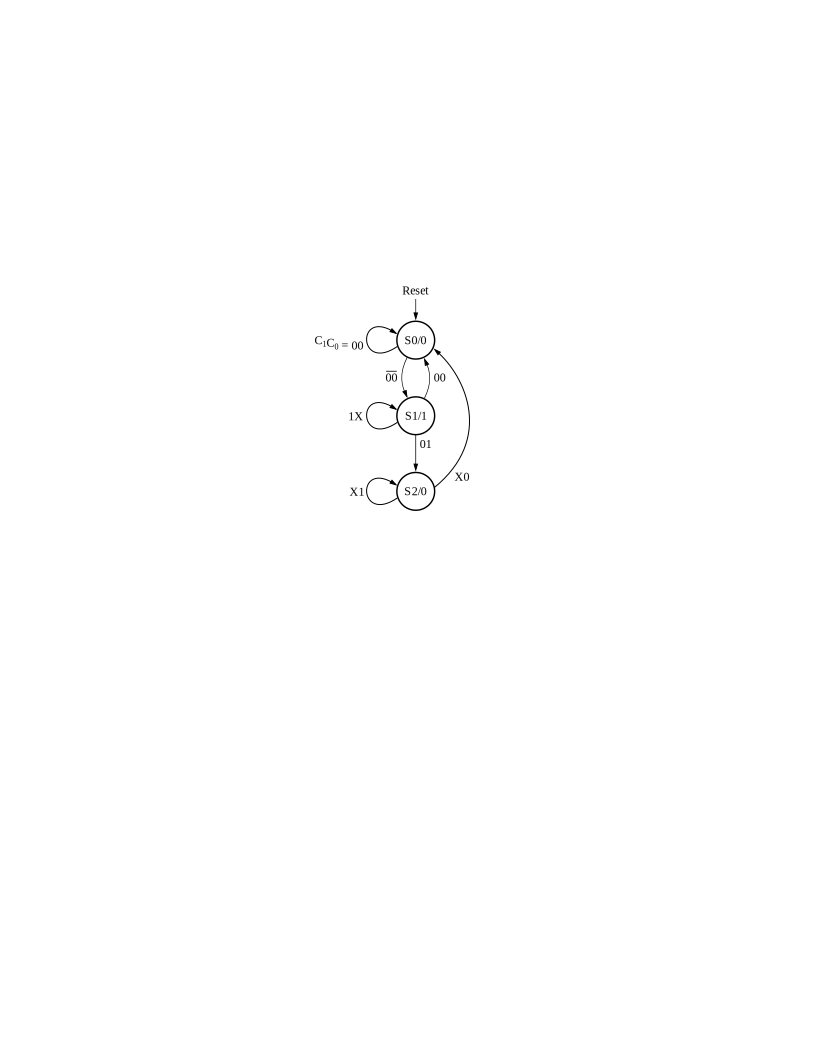
\includegraphics[scale=1.0]{figures/fsm.pdf}
   \end{center}
   \caption{A finite state machine controller.}
	\label{fig:fsm}
\end{figure}

\noindent
The FSM in Figure~\ref{fig:fsm} starts in the 
state S0 and produces the output $z = 0$, which is indicated in the state diagram
as S0/0. As long as $C_1 C_0 = 00$ the FSM remains in S0. Consider now the
case where $C_1$ changes to 1. On the next active clock edge the FSM transitions to
state S1, where it produces $z=1$ to enable the LFSR. The FSM remains in this state
as long as $C_1 = 1$, as indicated by the arrow labeled 1X (the value 1X
represents both of the cases $C_1 C_0 = 10$ and $C_1 C_0 = 11$). This scenario puts the LFSR
in the {\it continuous} operating mode, where it will generate a new random integer for
each clock cycle.  When $C$ changes back to
00 the FSM transitions back to the starting state S0. Next, consider the case when
$C_1 = 0$ but $C_0$ changes to 1. On the next active clock edge the FSM changes 
to state S1, setting $z=1$, but it remains in this state for only one clock cycle.
Following the arrow labeled $C_1 C_0 = 01$ the subsequent clock edge causes the 
FSM to move to state S2, where $z=0$. As long as $C_0 = 1$ the FSM will remain
in S2, and will return to S0 when $C_0$ changes to 0. Since this scenario causes 
the LFSR to generate exactly one new random integer, it implements the
{\it step} operating mode.

~\\
\noindent
A diagram of the Application Logic circuit is shown in Figure~\ref{fig:appl}. It includes 
a two-bit address input $A$, an $n$-bit data input $D$, and a write input $W$ that represent 
the way this circuit will (in Part II) be included in an AFU and connected to a processor. 
The address decoding, which is done using NOR gates, assigns the address $A_1 A_0 = 00$ to 
the polynomial register, $A_1 A_0 = 01$ to the LFSR register, and $A_1 A_0 = 10$ to the 
control register. The AND gates in the circuit ensure that each register can be loaded with
the data $D$ when its address is selected and $W=1$. When data is written to the LFSR it
is loaded into the seed input $S$; the LFSR enable input $E$ is controlled by the $z$ output 
of the FSM. 

\begin{figure}[ht]
   \begin{center}
       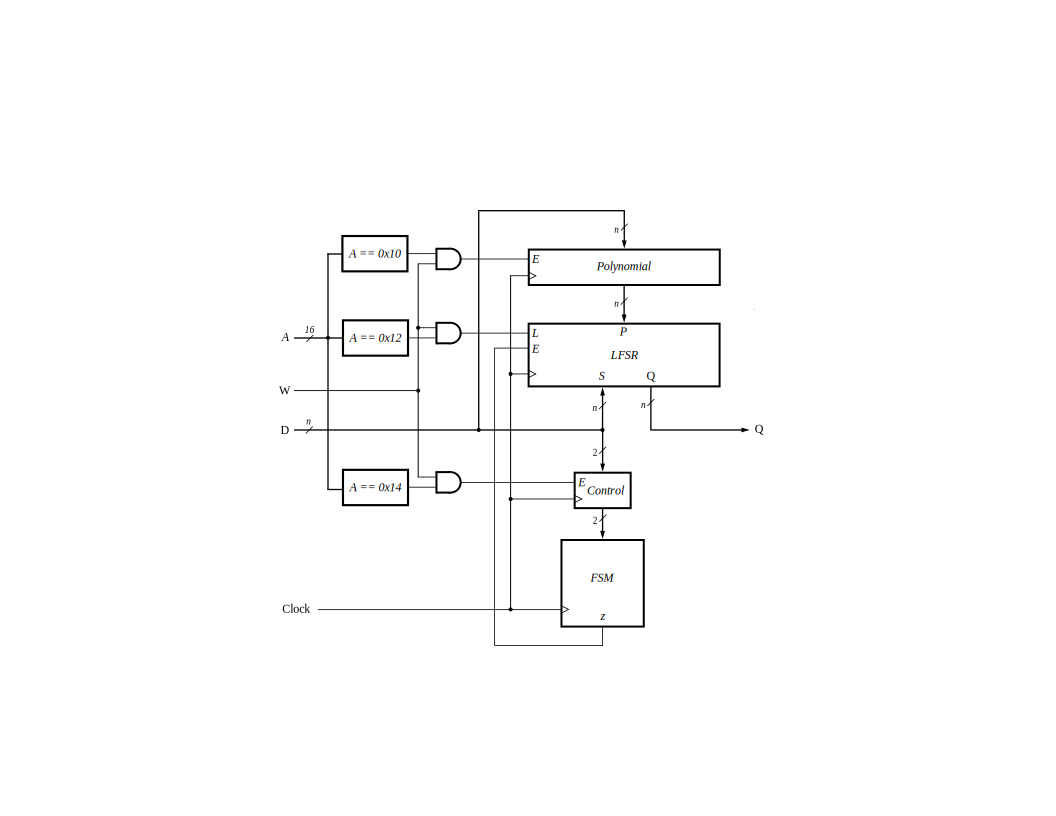
\includegraphics[scale=1.0]{figures/application.pdf}
   \end{center}
   \caption{The application logic circuit.}
	\label{fig:appl}
\end{figure}

~\\
\noindent
Perform the following steps to complete the design of the Application Logic module 
with Verilog code:

\begin{enumerate}
\item
You should design your Verilog code on a ``home'' computer of your choosing. 
No tools on the DevCloud are needed for this part of the exercise. To compile and simulate
your Verilog code we assume that you have access to a Verilog simulator, such as 
the {\it ModelSim} simulator. Although any modern Verilog simulator can be used, the specific
version that we refer to in the discussion below is called 
{\it ModelSim-Intel FPGA Starter Edition 2020.1}. If needed, you can download and 
install a {\it free} version of this simulator from Intel's website (any recent version of
the software can be used). An introduction to this simulator can be found in 
the tutorial {\it Using the ModelSim-Intel FPGA Simulator with Verilog Testbenches}.
This tutorial is available on the Internet from the Intel FPGA Academic Program.
\item
Make a new folder on your computer for this part of the exercise. Create a Verilog
source-code file named {\it application.sv} (the {\it sv} filename extension enables the 
use of System Verilog extensions), and write the code for the circuit in 
Figure~\ref{fig:appl}. A template for this Verilog code is shown in Figure~\ref{fig:code}.

\begin{figure}[H]
\begin{center}
\lstset{language=Verilog,morekeywords={logic,always_ff,endmodule},numbers=none,escapechar=|}
\lstinputlisting{../design_files/hw/part1/application.sv}
\end{center}
\caption{A template for the Application Logic Verilog code.}
\label{fig:code}
\end{figure}

\item
Simulate your code to ensure that it works correctly. Example results produced by using
{\it ModelSim} for a correctly-designed circuit are given in Figures~\ref{fig:cont}
and~\ref{fig:step}. For convenience of reference, the simulation is based on a clock 
waveform with a 10 ns period. After resetting the circuit 
(each register has an active-high synchronous reset 
capability), the simulation loads initial values into the three registers in the circuit. 
On the clock edge at 15 ns in simulation time the polynomial register is loaded with the
value 221. In the subsequent clock cycle a seed value of 1 is loaded into the LFSR register. 
Then, the clock edge at 35 ns sets the control register to $C_1 C_0 = 10$, causing the 
FSM to enter the {\it continuous} operating mode in state S1 at 45 ns.
Note that Q $= P = 221$ after the clock edge at 55 ns, which is the 
result of setting the seed to the value 1.  Over the next few clock cycles, as shown 
in Figure~\ref{fig:cont}, the LFSR produces a sequence of ``random'' integers. 
At 135 ns the simulation loads the control register with $C_1 C_0 = 00$, which causes the 
FSM to change back to state~S0.

~\\
\begin{figure}[h]
   \begin{center}
       \includegraphics[width=\textwidth]{figures/lfsr_cont.png}
   \end{center}
   \caption{Using the LFSR in continuous mode.}
	\label{fig:cont}
\end{figure}

~\\
\noindent
Figure~\ref{fig:step} continues the simulation results from Figure~\ref{fig:cont}. At 155 ns
the seed value in the LFSR is reinitialized to~1. Then, in the next clock cycle the control 
register is set to $C_1 C_0 = 01$, causing the FSM to enter {\it step} mode by transitioning 
through state S1 to S2. The control register is set back to $C_1 C_0 = 00$ at 185 ns, so that the
FSM moves back to state S0 at 195 ns. Finally, the step mode is used to generate a 
few more ``random'' values as shown in the remainder of the simulation. The sequence of 
integers generated in Figures~\ref{fig:cont} and~\ref{fig:step} are identical, because they 
are derived from the same seed and polynomial. Due to this behavior, an LFSR is said to 
generate integers that are {\it pseudo} random.

\begin{figure}[h]
   \begin{center}
       \includegraphics[width=\textwidth]{figures/lfsr_step.png}
   \end{center}
   \caption{Using the LFSR in step mode.}
	\label{fig:step}
\end{figure}
\end{enumerate}

\noindent
The simulation results from Figures~\ref{fig:cont} and~\ref{fig:step} are based on the
Verilog {\it testbench} shown in Figure~\ref{fig:tb}. This testbench and the template code
in Figure~\ref{fig:code} are provided for your use along with this laboratory exercise.

\lstset{language=Verilog,numbers=none,escapechar=|}
\begin{figure}[H]
\begin{center}
\begin{minipage}[h]{15 cm}
\begin{lstlisting}[name=code]
`timescale 1ns / 1ps

module testbench ( );
    reg reset, clock, W;                // declare design under test (DUT) inputs
    reg [15:0] A;                       // address
    reg [7:0] D;                        // data
    wire [7:0] Q;                       // declare DUT outputs

    application U1 (reset, clock, W, A, D, Q); // instantiate the DUT

    // define a 100 MHz clock waveform
    always
        #5 clock <= ~clock;
    
    // assign inputs at various times
    initial 
    begin
        clock <= 1'b0;
        reset <= 1'b1;
        W <= 1'b0; A <= 2'bXX;
        #10  reset <= 1'b0;             // initialize the polynomial
             A <= 16'h0010; D <= 221; W <= 1'b1;
        #10  A <= 16'h0012; D <= 1'b1;  // initialize the seed
        #10  A <= 16'h0014; D <= 2'b10; // Set CTRL to continuous mode
        #10  W <= 1'b0;
        #90  D <= 0; W <= 1'b1;         // set CTRL to stopped mode
        #20  A <= 16'h0012; D <= 1;     // re-initialize the seed
        #10  A <= 16'h0014; D <= 8'b01; // set CTRL to step mode
        #20  D <= 8'b00;   // stop
        #10  D <= 8'b01;   // step
        #20  D <= 8'b00;   // stop
        |$\ldots$|
    end // initial
endmodule
\end{lstlisting}
\end{minipage}
\caption{The simulation testbench.}
\label{fig:tb}
\end{center}
\end{figure}
\section*{Part II}
In this part of the exercise we will augment the application logic circuit from Part I 
to create an AFU that can be connected to a processor. This step will require the
design of some additional Verilog code, as well as the use of
a number of hardware development tools that are provided on the DevCloud.
As indicated in Figure~\ref{fig:block} an AFU has a {\it protocol} port and some logic for
reading and writing registers based on this protocol. For this exercise we will use the
{\it Core Cache Interface} Protocol (CCI-P) that is provided by Intel. This protocol
is part of the FIU interface in Figure~\ref{fig:block} and 
defines a signaling convention for connecting the processor and AFU. 

~\\
\noindent
Figure~\ref{fig:AFU_code} provides a template for your AFU Verilog module.
In Part $a$ of the figure, 
Lines~\ref{line:platform} and~\ref{line:json} {\it include} the Verilog {\it header}
files {\it platform\_if.vh} and {\it afu\_json\_info.vh}. The first of these files defines
some CCI-P data types that are used in the code, and the second one specifies some key 
information about your AFU.  We will discuss the contents of {\it afu\_json\_info.vh} shortly.

~\\
\noindent
Your AFU module is required to have the name {\it afu}, as given in the figure. Depending
on its functionality, an AFU may have different ports. In our case, in addition to 
{\it clock} and {\it reset} inputs, we require an input, called {\it rx}, for receiving CCI-P 
data, and an output, named {\it tx}, for transmitting data. These {\it rx} and {\it tx} ports 
have special data types, shown in Lines~\ref{line:rx} and~\ref{line:tx}, that are defined 
via the header file {\it platform\_if.vh}.

\lstset{language=Verilog,morekeywords={enum,logic,always_ff},numbers=left,escapechar=|}
\begin{figure}[H]
\begin{center}
\begin{minipage}[h]{15 cm}
\begin{lstlisting}[name=AFU]
|\label{line:platform}|`include "platform_if.vh"
|\label{line:json}|`include "afu_json_info.vh"

module afu (clock, reset, rx, tx);
    input  clock;                   // CCI-P clock
    input  reset;                   // CCI-P reset
    |\label{line:rx}|input  t_if_ccip_Rx rx;         // receive channel
    |\label{line:tx}|output t_if_ccip_Tx tx;         // transmit channel

    |\label{line:n}|parameter n = 32;
    logic [n-1:0] Q, Poly;          // LFSR and polynomial registers
    logic [1:0] Ctrl;               // control register
    logic [15:0] A;                 // Address
    |\label{line:D}|logic [n-1:0] D;                // Data
    |\label{line:W}|logic W;                        // Write signal
    |$\ldots$| declare other signals

    |\label{line:h1}|t_ccip_c0_ReqMmioHdr mmioHdr;   // channel c0 header
    |\label{line:h2}|assign mmioHdr = t_ccip_c0_ReqMmioHdr'(rx.c0.hdr);

    |\label{line:A}|assign A = mmioHdr.address;     // rename address signal
    assign D = rx.c0.data;          // rename data signal
    assign W = rx.c0.mmioWrValid;   // rename write signal

    |\label{line:poly}|always_ff @(posedge clock)      // the polynomial register
        if (reset)
            Poly <= '0;
        else if (W && A == 16'h0010)
            Poly <= D;  // set the polynomial

    |$\ldots$| define the LFSR
    |$\ldots$| define the control register
    |$\ldots$| define the finite state machine
\end{lstlisting}
\end{minipage}
\caption{A template for the AFU Verilog code (Part $a$).}
\label{fig:AFU_code}
\end{center}
\end{figure}

\lstset{language=Verilog,morekeywords={enum,logic,always_ff},numbers=left,escapechar=|}
\begin{minipage}[t]{15.5 cm}
\begin{lstlisting}[name=AFU]
    |\label{line:afu_id}|logic [127:0] afu_id = `AFU_ACCEL_UUID; // from afu_json_info.vh

    always_ff @(posedge clock) begin // respond to memory-mapped I/O reads
        if (reset) begin
            tx.c1.hdr <= '0;
            tx.c1.valid <= '0;
            tx.c0.hdr <= '0;
            tx.c0.valid <= '0;
            tx.c2.hdr <= '0;
            tx.c2.mmioRdValid <= '0;
        end
        else begin
            // clear read response flag in case there was a response last cycle
            tx.c2.mmioRdValid <= 0;

            // serve MMIO read requests
            if (rx.c0.mmioRdValid == 1'b1) begin
                // copy TID, which host needs to map response to request
                tx.c2.hdr.tid <= mmioHdr.tid;
                // post response
                tx.c2.mmioRdValid <= 1;

                |\label{line:case}|case (A)
                    // AFU header
                    16'h0000: tx.c2.data <= {
                        4'b0001, // Feature type = AFU
                        8'b0,    // reserved
                        4'b0,    // afu minor revision = 0
                        7'b0,    // reserved
                        1'b1,    // end of DFH list = 1
                        24'b0,   // next DFH offset = 0
                        4'b0,    // afu major revision = 0
                        12'b0    // feature ID = 0
                    };
                    16'h0002: tx.c2.data <= afu_id[63:0];   // AFU_ID_L
                    16'h0004: tx.c2.data <= afu_id[127:64]; // AFU_ID_H
                    16'h0006: tx.c2.data <= 64'h0;          // DFH_RSVD0
                    16'h0008: tx.c2.data <= 64'h0;          // DFH_RSVD1

                    // application logic registers
                    |\label{line:polyr}|16'h0010: tx.c2.data <= 64'(Poly);
                    |\label{line:Q}|16'h0012: tx.c2.data <= 64'(Q);
                    |\label{line:ctrl}|16'h0014: tx.c2.data <= 64'(Ctrl);

                    default:  tx.c2.data <= 64'h0;
                endcase
            end
        end
    end
endmodule
\end{lstlisting}
\begin{center}
Figure \ref{fig:AFU_code}. A template for the AFU Verilog code (Part $b$).
\end{center}
\end{minipage}

~\\
~\\
\noindent
In Lines~\ref{line:n} to~\ref{line:W} the code sets the parameter $n=32$ and declares a
number of signals. The signal Q represents the LFSR in Figure~\ref{fig:appl}. For the 
Verilog code in Figure~\ref{fig:code} the signal Q served as the output of the module, but 
for the AFU the processor reads the contents of registers via the {\it tx} output port.

~\\
\noindent
Lines~\ref{line:h1} and~\ref{line:h2} declare a special type of CCI-P signal called 
{\it mmioHdr}. This signal provides the {\it address} of the register currently being 
accessed by the processor, which is assigned to the 16-bit signal $A$ in Line~\ref{line:A}. 
The address is implemented in the CCI-P as an {\it offset} from a {\it base} address 
that is used for memory-mapped I/O. Each address $A$ is aligned to a double-word (32-bit) 
boundary in the processor's address space. Lines~\ref{line:D} and~\ref{line:W}
assign the processor $n$-bit {\it data} signal and {\it write} control signal to the 
variables $D$ and $W$, respectively. These signals are valid whenever the processor is 
performing a {\it write} to a register in the AFU. 

~\\
\noindent
Using the polynomial register as an example, the {\it always} block 
in Line~\ref{line:poly} shows how registers can be defined in the AFU. Note that this code 
is very similar to that from Figure~\ref{fig:code}. 

~\\
\noindent
Part $b$ of Figure~\ref{fig:AFU_code} gives mandatory code that must be present in an AFU 
to support read operations from the processor at specific addresses. These addresses are decoded
in the AFU by using the {\it case} statement in Line~\ref{line:case}. As shown, each
address responds by placing data onto the {\it tx} output of the AFU. For address $A = 0$
the AFU responds with a particular 64-bit data pattern that is required for any AFU. Addresses
$A=2$ and $A=4$ respond with the low and high 64-bits of the {\it afu\_id} signal. This signal
represents a globally-unique identifier for the AFU. It is declared in Line~\ref{line:afu_id}
and initialized with the symbolic constant \texttt{AFU\_ACCEL\_UUID}, which is
defined in the file {\it afu\_json\_info.vh}.  Finally, addresses $A=6$ and $A=8$
respond with 0 for our AFU.  More details about the mandatory addresses that have to be
supported in an AFU can be found by searching online for documentation related to CCI-P.

~\\
\noindent
Lines~\ref{line:polyr} to~\ref{line:ctrl} allow the processor to read the contents of the 
polynomial register, LFSR, and control register at the addresses $A=(10)_{16}$, $A=(12)_{16}$,
and $A=(14)_{16}$, respectively. As mentioned previously, each address $A$ represents a
double-word (32 bit) processor address. This means that the addresses decoded in our case
statement are aligned to a quad-word (64 bit) boundary, because the least-significant 
address bit $A_0 =0$ for each address. The CCI-P specification requires this alignment 
for all registers in an AFU.

~\\
\noindent
Perform the following steps to complete the design of the AFU:

\begin{enumerate}
\item
Make a new folder on your home computer called \texttt{lfsr\_afu}. Then, in this folder create two
subfolders named \texttt{hw} and \texttt{sw}. The \texttt{sw} folder will be used in 
Parts 3, 4, and 5 of this exercise. Now, in the \texttt{hw} folder make a subfolder 
called \texttt{rtl}. You should now have created the folders illustrated in 
Figure~\ref{fig:folders}. This arrangement of folders is required when using the compilation 
tools that are provided on the DevCloud.
\item
In your \texttt{rtl} subfolder, make a new Verilog source-code file called 
{\it afu.sv}. Enter the code from Figure~\ref{fig:AFU_code} into this file and, as indicated 
in Part $a$ of the figure, fill in the code that is needed to define the LFSR, control register, 
and finite state machine.  Note that the code shown in Figure~\ref{fig:AFU_code} is provided
for you in the file {\it afu.sv} that is part of the {\it design\_files} material included 
along with this exercise.

~\\
\begin{figure}[h]
   \begin{center}
       \includegraphics[]{figures/folders.pdf}
   \end{center}
   \caption{The arrangement of folders for an AFU.}
	\label{fig:folders}
\end{figure}

\item
To compile the Verilog code for your AFU, the development tools on the DevCloud require
several files in addition to {\it afu.sv}. The names of the 
required files have to be listed in a
{\it plain-text} file named {\it filelist.txt} in the \texttt{rtl} folder. The contents of 
this file for our AFU is shown in Figure~\ref{fig:filelist}. The first file listed is 
{\it lfsr\_afu.json}, which gives some important information about the AFU in 
{\it JavaScript Object Notation} (JSON) format. As shown in
Figure~\ref{fig:json}, this JSON file specifies the type of CCI-P port used for the
AFU, which is called {\it ccip\_std\_afu}. This interface consists of 
{\it clock}, {\it reset}, receive ({\it rx}) and transmit ({\it tx}) ports, as given 
in Figure~\ref{fig:AFU_code}. The JSON file also specifies the AFU name, 
{\it lfsr\_afu}, and its {\it Universally Unique Identifier} (UUID). The UUID shown in the
figure is just a placeholder; we will generate a new UUID for the AFU by using the
{\it uuidgen} command that is available on the DevCloud. The Verilog source-code files listed in
{\it filelist.txt} specify the AFU and its CCI-P interface. The files
{\it ccip\_interface\_reg.sv} and {\it ccip\_std\_afu.sv} have to be present in the AFU's 
\texttt{rtl} folder.

~\\
\noindent
The files {\it filelist.txt}, {\it lfsr\_afu.json}, {\it ccip\_interface\_reg.sv}, and 
{\it ccip\_std\_afu.sv} are provided for you as part of the {\it design\_files}
that are included with this exercise. Copy these files into your \texttt{rtl} folder, to
create the structure of files illustrated in Figure~\ref{fig:files}.

\lstset{language=C,numbers=none,escapechar=|}
\begin{figure}[H]
\begin{center}
\begin{minipage}[h]{4.5 cm}
\begin{lstlisting}[name=filelist]
lfsr_afu.json

afu.sv
ccip_interface_reg.sv
ccip_st_afu.sv
\end{lstlisting}
\end{minipage}
\caption{The contents of {\it filelist.txt}.}
\label{fig:filelist}
\end{center}
\end{figure}

\lstset{language=Java,numbers=none,escapechar=|}
\begin{figure}[H]
\begin{center}
\begin{minipage}[h]{15 cm}
\begin{lstlisting}[name=json]
{
    "version": 1,
    "afu-image": {
        "power": 0,
        "afu-top-interface": {
            "class": "ccip_std_afu"
        },
        "accelerator-clusters": [
            {
                "name": "lfsr_afu",
                "total-contexts": 1,
                "accelerator-type-uuid": "850adcc2-6ceb-4b22-9722-d43375b61c66"
            }
        ]
    }
}
\end{lstlisting}
\end{minipage}
\vspace{-.5cm}
\caption{The JSON file.}
\label{fig:json}
\end{center}
\end{figure}

\item
For the remainder of this exercise we assume that you are able to login to the DevCloud
and configure the environment variables and settings that are needed for AFU development. 
To perform this step it is important to be familiar with the material presented in the
tutorial {\it Using the Intel FPGA DevCloud for AFU Development}. First, 
copy the folders and files shown in Figure~\ref{fig:files} onto the DevCloud.  Then, 
using the Linux command line interface on the DevCloud execute the command 
\texttt{uuidgen} to generate a new UUID for the LFSR AFU.
Enter this new UUID into the file {\it lfsr\_afu.json}, replacing the placeholder given in
Figure~\ref{fig:json}.

\item
On the DevCloud, set your working directory to the \texttt{lfsr\_afu} folder, and then 
run the command: 

\noindent
\texttt{afu\_synth\_setup -s hw/rtl/filelist.txt build\_synth}

Now, change your working directory to the newly-created \texttt{build\_synth} folder and 
execute the command \texttt{run.sh}. This command uses the information in 
the {\it lfsr\_afu.json} file to generate the Verilog header file {\it afu\_json\_info.vh}, 
which is included in the code shown in Figure~\ref{fig:AFU_code}. 
The \texttt{run.sh} command then executes the Intel 
Quartus\textsuperscript{\textregistered} Prime software to compile the AFU into a circuit
that can be implemented in the target FPGA device.

~\\
\noindent
The Quartus Prime software begins by executing its synthesis tools that
compile your Verilog source code. If any syntax errors are reported (they are shown in 
\red{red}), then fix these errors and compile again. Note that it is 
``normal'' to receive a significant number of warning messages from the Quartus Prime 
software when compiling an AFU; while you should still monitor these messages, those that
refer to code that is not part of your {\it afu.sv} file can usually be ignored.

~\\
\noindent
After successful compilation of your AFU code, the Quartus Prime software generates an FPGA 
programming bit-stream file called {\it lfsr\_afu.gbs}. In Intel\textsuperscript{\textregistered}
FPGA literature, this type of file is known as a {\it Green Bitstream} and represents a 
{\it partial-reconfiguation} file for the target FPGA. You can download this {\it gbs} file 
into the FPGA device on the DevCloud, where it joins the main bit-stream that is 
already present in the FPGA. Intel refers to the main bit-stream as the {\it Blue Bitstream}. 
To download your AFU into the FPGA execute the command:

\noindent
\texttt{fpgasupdate lfsr\_afu.gbs}.

Note that if you are using version 1.2.1 of the Arria 10 Development Stack on the
DevCloud, then you have to execute two commands to program the FPGA. First, execute:

\noindent
\texttt{PACSign PR -t UPDATE -H openssl\_manager -i lfsr\_afu.gbs -o lfsr\_afu\_unsigned.gbs}

\noindent Type \texttt{y} ({\it yes}) in answer to the queries that are issued by this command. 
Then, execute:

\noindent
\texttt{fpgasupdate lfsr\_afu\_unsigned.gbs}.
\end{enumerate}

\begin{figure}[t]
   \begin{center}
       \includegraphics[]{figures/files.pdf}
   \end{center}
   \caption{The files needed for an AFU.}
	\label{fig:files}
\end{figure}

~\\
\noindent
Now that the AFU has been downloaded into the target FPGA device, we can develop software 
programs which run on the processor and make use of the AFU.

\section*{Part III}
For the development of software for AFUs Intel provides a collection of open-source
utilities known as the {\it Open Programmable Acceleration Engine} (OPAE).  An example of 
a C program that uses the OPAE infrastructure to access the AFU developed in this exercise 
is given in Figure~\ref{fig:C_code}. This code includes the OPAE header file {\it mmio.h},
which is required to perform memory-mapped I/O.

\lstset{language=C,numbers=left,escapechar=|}
\begin{figure}[H]
\begin{center}
\begin{minipage}[h]{15 cm}
\begin{lstlisting}[name=C_code]
#include <stdio.h>
#include <opae/mmio.h>

// Application Logic register addresses (offsets)
|\label{line:a1}|#define POLY_REG    0X10 << 2
#define LFSR_REG    0X12 << 2
|\label{line:a2}|#define CTRL_REG    0X14 << 2

|\label{line:open}|int open_AFU (fpga_handle *);
|\label{line:close}|void close_AFU (fpga_handle);

int main(int argc, char *argv[])
{
    |\label{line:handle}|fpga_handle handle = NULL;
    if (open_AFU (&handle) < 0)
        return -1;

    uint32_t data;
    (void) fpgaWriteMMIO32 (handle, 0, POLY_REG, 221);   // set polynomial
    (void) fpgaReadMMIO32 (handle, 0, POLY_REG, &data);  // set seed
    printf ("Polynomial set to: %d\n", data);
    
    (void) fpgaWriteMMIO32 (handle, 0, LFSR_REG, 0x1);
    (void) fpgaReadMMIO32 (handle, 0, LFSR_REG, &data);
    printf ("Seed set to: %d\n", data);

    bool found[256] = { false };
    bool stop = false;
    int length = 0;
    |\label{line:while}|while (!stop) {
        if (found[data]) stop = true;
        else {
            ++length;
            found[data] = true;

            // get a new random integer from the LFSR // 
            (void) fpgaWriteMMIO32 (handle, 0, CTRL_REG, 0x1);  // step
            (void) fpgaWriteMMIO32 (handle, 0, CTRL_REG, 0x0);  // stop
            (void) fpgaReadMMIO32 (handle, 0, LFSR_REG, &data);
            printf ("LFSR: %d\n", data);
        }
    }
    printf("\nLength of random sequence: %d\n", length);

    close_AFU (handle);
    return 0;
}
\end{lstlisting}
\end{minipage}
\caption{Using the AFU in a C program.}
\label{fig:C_code}
\end{center}
\end{figure}

\noindent
Lines~\ref{line:a1} to~\ref{line:a2} in Figure~\ref{fig:C_code} define the addresses 
that software has to use to
access the polynomial, LFSR, and control registers in the ALU. These addresses are the
same as the ones given in Figure~\ref{fig:AFU_code}, except that they are shifted left by 
two bit positions. This bit-shifting is done to convert the double-word (32-bit aligned)
addresses used in the Verilog code to byte addresses that are issued by the processor.

~\\
\noindent
In Lines~\ref{line:open} and~\ref{line:close} prototypes are given for the functions 
{\it open\_AFU} and {\it close\_AFU}. The first of these functions sets up a communication 
mechanism between the software program and the AFU, via a Linux device driver. The second
function terminates this connection. The {\it open\_AFU} function calls several OPAE library
utilities to check if the AFU is available and working properly. If so, the {\it handle} 
variable, declared with the OPAE type {\it fpga\_handle} in Line~\ref{line:handle}, is 
set up as a {\it pointer} to the AFU. The {\it open\_AFU} function uses this pointer to 
``print'' to the Linux Terminal the contents of the mandatory register addresses in the AFU,
which are specified in Figure~\ref{fig:AFU_code}. Appendix~A shows the source code for
{\it open\_AFU}, in Figure~\ref{fig:open_AFU}. If it is able to communicate successfully with 
the AFU then the function returns 0, otherwise it returns -1. 
Figure~\ref{fig:print} in Appendix A displays the code for the function {\it print\_AFU\_regs}, 
which is called by {\it open\_AFU}, and the code for {\it close\_AFU} is given in
Figure~\ref{fig:close}.

~\\
\noindent
The remainder of the code in Figure~\ref{fig:C_code} uses memory-mapped I/O via the {\it handle}
variable to access the registers in the LFSR AFU. 
The {\it fpgaReadMMIO32} function allows the software to
read the contents of an AFU register, whereas {\it fpgaWriteMMIO32} allows a new value 
to be written to a register. 
The purpose of the software code is to use the {\it while} loop in Line~\ref{line:while} 
to cause the LFSR to reproduce the sequence 
of random integers that is illustrated in the simulation results in
Figures~\ref{fig:cont} and~\ref{fig:step}. The while loop exits when the LFSR produces a
value that is a duplicate of a previous one, marking the end of the sequence. 

~\\
\noindent
To complete this part of the exercise perform the following steps:

\begin{enumerate}
\item
A file named {\it part3.c} that contains the code from Figure~\ref{fig:C_code}, and a file 
named {\it manage\_afu.c}, which holds the C code for {\it open\_AFU} and {\it close\_AFU},
are included in the {\it design\_files} that accompany this exercise.
Copy these files into the \texttt{sw} folder for the AFU on the DevCloud.
\item
To compile the code in {\it part3.c} and {\it manage\_AFU.c} you have to use a special 
{\it Makefile} that employs the OPAE infrastructure on the DevCloud. Copy this {\it Makefile}, 
which is also included in the {\it design\_files} for this exercise, into your \texttt{sw} folder. 
\item
In the \texttt{sw} directory on the DevCloud run the command \texttt{make part3}. The
results are displayed in Figure~\ref{fig:output}. As shown in the figure,
one of the programs executed by \texttt{make} is {\it afu\_json\_mgr}. This
program reads the file {\it lfsr\_afu.json} shown in Figure~\ref{fig:json} to find the 
UUID for the AFU, and then produces the C header file {\it afu\_json\_info.h}. This header
file is used by {\it manage\_afu.c}. To execute your program type \texttt{./part3}, 
as illustrated in Figure~\ref{fig:output}.
\end{enumerate}

\section*{Part IV}
As shown in Figure~\ref{fig:output} the program from Part III produces a sequence of 
15 random values based on the
polynomial $P = 221$ and starting with the seed value $S = 1$.  In general, an LFSR may
produce sequences of varying lengths depending on the polynomial and seed combination. For
an $n$-bit LFSR a polynomial that results in a maximal sequence length, which is $2^n -1$
different values, is known as a {\it primitive} polynomial. For this part of the exercise
you are to write a C program that employs your LFSR AFU to find all eight-bit primitive
polynomials. The smallest polynomial to consider is $P = (80)_{16} = 128$ and the largest
is $P = (\mathrm{FF})_{16} = 255$.

~\\
\noindent Perform the following:

\begin{enumerate}
\item
Write your C code in a file {\it part4.c}, making use of the functions {\it open\_AFU} and
{\it close\_AFU} as shown in Figure~\ref{fig:C_code}. For each polynomial of interest 
set the seed value to $S = 1$ and determine the resulting sequence length.  Control the 
LFSR using step mode so that you can generate one random value at a time. You should
display the value of each primitive polynomial on the Linux Terminal window. Also display
the sequence of random values produced by each of these polynomials, starting and ending
with the seed value $S = 1$.
\item
To compile your code on the DevCloud, put {\it part4.c} into your \texttt{sw} folder and 
execute \texttt{make part4}.
\end{enumerate}

\lstset{language=C,morekeywords={u42132@s005-n005,LFSR},numbers=none,escapechar=|}
\begin{figure}[H]
\begin{center}
\begin{minipage}[h]{\textwidth}
\begin{lstlisting}[name=output]
|\green{userid@s005-n005}:\blue{~/lfsr\_afu/sw}|$ ls
Makefile  manage_afu.c  manage_afu.o  part3.c
|\green{userid@s005-n005}:\blue{~/lfsr\_afu/sw}|$ make part3
afu_json_mgr json-info --afu-json=../hw/rtl/lfsr_afu.json --c-hdr=afu_json_info.h
Writing afu_json_info.h
gcc -fstack-protector -fPIE -fPIC -O2 -D_FORTIFY_SOURCE=2 -Wformat -Wformat-security -Werror -g -O2 -std=c99 -Wall -Wno-unknown-pragmas -c -o part3.o part3.c
gcc -fstack-protector -fPIE -fPIC -O2 -D_FORTIFY_SOURCE=2 -Wformat -Wformat-security -Werror -g -O2 -std=c99 -Wall -Wno-unknown-pragmas -c -o manage_afu.o manage_afu.c
gcc -fstack-protector -fPIE -fPIC -O2 -D_FORTIFY_SOURCE=2 -Wformat -Wformat-security -Werror -g -O2 -std=c99 -Wall -Wno-unknown-pragmas -o part3 part3.o manage_afu.o -z noexecstack -z relro -z now -pie -luuid -lpthread -lopae-c
|\green{userid@s005-n005}:\blue{~/lfsr\_afu/sw}|$ ls
afu_json_info.h  Makefile  manage_afu.c  manage_afu.o  part3  part3.c  part3.o
|\green{userid@s005-n005}:\blue{~/lfsr\_afu/sw}|$ ./part3
Opening lsfr_afu
AFU DFH REG  = 0x1000010000000000
AFU ID HI    = 0x8031be250cf440ee
AFU ID LO    = 0xa411dbaf7e894df5
AFU NEXT     = 0x0000000000000000
AFU RESERVED = 0x0000000000000000
Polynomial set to: 221
Seed set to: 1
LFSR: 221
LFSR: 179
LFSR: 132
LFSR: 66
LFSR: 33
LFSR: 205
LFSR: 187
LFSR: 128
LFSR: 64
LFSR: 32
LFSR: 16
LFSR: 8
LFSR: 4
LFSR: 2
LFSR: 1

Length of random sequence: 15
|\green{userid@s005-n005}:\blue{~/lfsr\_afu/sw}||\$|
\end{lstlisting}
\end{minipage}
\caption{Compiling and executing {\it part3.c}.}
\label{fig:output}
\end{center}
\end{figure}

\section*{Part V}

In this part of the exercise you will utilize the LFSR AFU to help create an animation.
Although the Linux Terminal normally displays ASCII text, we can use the 
Terminal's {\it escape commands} to make simple drawings, often called 
{\it ASCII graphics}. Animations can be created on the Terminal by using commands to 
clear the screen, move the Terminal cursor to specific locations, show/hide the cursor, 
change the color of characters, and so on. An example of a program that uses ASCII graphics is 
given in Figure~\ref{fig:dots}. 
It first {\it includes} the {\it stdio.h} library and then 
defines constants, described later, for text colors which can be used in the Terminal window. 

\lstset{language=C,numbers=left,escapechar=|}
\begin{figure}[h]
\begin{center}
\begin{minipage}[t]{12.5 cm}
\begin{lstlisting}[name=dots]
|\label{line:includes}|/* This program draws a few characters on the screen. */
#include <stdio.h>
#define YELLOW 33
#define CYAN 36
#define WHITE 37

void plot_pixel(int, int, char, char);

int main(void) {
    int i;
    |\label{line:clear}|printf ("\e[2J");            // clear the screen
    |\label{line:hide}|printf ("\e[?25l");          // hide the cursor

    |\label{line:plot1}|plot_pixel (1, 1, CYAN, 'X');
    plot_pixel (12, 12, CYAN, 'X');
    for (i = 2; i < 12; ++i)
        |\label{line:plot2}|plot_pixel (6, i + 12, YELLOW, '*');

    |\label{line:getchar}|(void) getchar ();           // wait for user to press return
    printf ("\e[2J");            // clear the screen
    |\label{line:reset}|printf ("\e[%2dm", WHITE);   // reset foreground color
    |\label{line:cursor}|printf ("\e[%d;%dH", 1, 1);  // move cursor to upper left
    |\label{line:show}|printf ("\e[?25h");          // show the cursor
    |\label{line:fflush}|fflush (stdout);
}

|\label{line:pp1}|void plot_pixel(int x, int y, char color, char c) {
    |\label{line:pixel}|printf ("\e[%2dm\e[%d;%dH%c", color, y, x, c);
    fflush (stdout);
|\label{line:pp2}|}
\end{lstlisting}
\end{minipage}
\caption{An example of code that uses ASCII graphics.}
\label{fig:dots}
\end{center}
\end{figure}

~\\
\noindent
A command is sent to the Terminal in line~\ref{line:clear} by using {\it printf}. All Terminal 
window commands begin with the ASCII \texttt{ESC} (escape) character, which is specified 
in the {\it printf} string using the syntax $\backslash$e. The command in line~\ref{line:clear},
which is \texttt{[2J}, instructs the Terminal to clear the screen. Another command, 
\texttt{[?25l}, given in line~\ref{line:hide}, causes the Terminal to {\it hide} the cursor 
so that it is not visible to the user. Next, the function \texttt{plot\_pixel} is called to draw
some characters at specific locations on the screen.  Coordinate $(1, 1)$ is at the top-left corner 
of the screen. The calls to \texttt{plot\_pixel} in
lines~\ref{line:plot1} to~\ref{line:plot2} draw cyan-colored \texttt{X} characters at
coordinates ($1, 1$) and ($12, 12$), and a vertical yellow line of ten \texttt{*} characters
along the sixth column.

~\\
\noindent The \texttt{plot\_pixel} function, shown in lines~\ref{line:pp1} to~\ref{line:pp2} uses 
two commands to draw a character. The first command is \texttt{[ccm}, where $cc$ is
called an {\it attribute}. The attribute can be used to set the color of text characters,
by using different values of $cc$. Examples of color attributes are $cc = 31$ (red), 
32 (green), 33 (yellow), 34 (blue), 35 (magenta), 36 (cyan), and 37 (white). The second command 
in \texttt{plot\_pixel} is \texttt{[yy;xxH}, where $yy$ and $xx$ specify a row and
column on the screen, respectively. This command moves the Terminal cursor to coordinate
$(xx, yy)$. In line~\ref{line:getchar} the program waits, using the \texttt{getchar}
function, for the user to press a key. Finally, commands are sent to the Terminal to {\it clear} 
the screen, {\it set} the color to white, {\it set} the cursor to coordinates ($1, 1$), and
{\it show} the cursor.

~\\
\noindent 
The use of ASCII graphics described above became popular around the year 1980 when they
were available in computer video terminals called the {\it VT100}, manufactured by Digital 
Equipment Corporation. The Linux Terminal provides ASCII graphics by {\it emulating} the 
capabilites of the VT100 video terminal. A listing of some escape commands is given in 
Appendix B. More information about ASCII graphics 
commands can be found by searching on the Internet for a topic such as ``VT100 graphics''.

~\\
\noindent
Perform the following:
\begin{enumerate}
\item Write C code using ASCII graphics to create an animation that ``prints'' random 
letters of the alphabet at random screen coordinates. The LFSR AFU should be used in
continuous mode to generate random integers over a 32-bit range. You can set the polynomial 
to $P = (b4bcd35c)_{16} = 3032273756$, which is a 32-bit primitive polynomial. Your code
should use random values from the LFSR to choose the letter to display, its color, and 
the $(x,y)$ screen coordinates. As an example, if the LFSR output is called {\it D}, then 
to randomly choose a letter $c$ from one of the five letters in the string ``intel'',
where 0 selects 'i', 1 select 'n', and so on, you can use the expression $c = D~\%~5$. 
The range of $x$ and $y$ coordinates produced by your program should cover 
the whole Terminal window.  Save your code in a file called {\it part5.c}.

\item
On the DevCloud compile your program by executing \texttt{make part5}. When you execute
the program by typing \texttt{./part5} the effect should be that every location in the Terminal 
window gets modified almost continuously. This result illustrates that the sequence of integers 
produced by the LFSR are sufficiently random for our purposes. To see an example of a
properly-working solution you can watch a {\it YouTube} video at
\texttt{https://youtu.be/JSbhbNVzNAY}. In this video the
animation selects a random letter from the string ``intel'' and prints it at a random
location on the screen, using a random color. The program is terminated by the user
pressing \^{}C. The video also shows a second animation in which ASCII graphics are used
to draw ``lines'' on the screen from one randomly-selected coordinate to another.
Lines that are mostly ``horizontal'' are drawn in blue, ``vertical'' lines in green, and 
diagonal lines in yellow or red. This program first draws a few lines slowly so that the 
user can see what is
happening, and then draws them as quickly as possible until the program is terminated.
\end{enumerate}

\newpage
\begin{center}\section*{Appendix A}\end{center}
\vspace{-1cm}
\lstset{language=C,numbers=none,escapechar=|}
\begin{figure}[H]
\begin{center}
\begin{minipage}[h]{\textwidth}
\begin{lstlisting}[name=manage]
#include <stdio.h>
#include <uuid/uuid.h>
#include <opae/enum.h>
#include <opae/access.h>
#include <opae/mmio.h>
#include <opae/properties.h>
#include <opae/utils.h>
#include "afu_json_info.h"

// mandatory AFU register addresses (offsets)
#define AFU_DFH_REG   0x0
#define AFU_ID_LO     0x8 
#define AFU_ID_HI     0x10
#define AFU_NEXT      0x18
#define AFU_RESERVED  0x20

int print_AFU_regs (fpga_handle);
fpga_properties filter = NULL;
fpga_token token = NULL;

int open_AFU (fpga_handle *handle) {
    fpga_guid guid;
    uint32_t num_matches;
    fpga_result res = FPGA_OK;

    char *AFU_NAME = AFU_ACCEL_NAME;    // from json file
    char *UUID = AFU_ACCEL_UUID;        // from json file
    printf ("Opening %s\n", AFU_NAME);
    if (uuid_parse(AFU_ACCEL_UUID, guid) < 0) {
        fprintf(stderr, "Error parsing guid '%s'\n", UUID);
        return -1;
    }
    if ((res = fpgaGetProperties (NULL, &filter)) != FPGA_OK) { // Look for AFU 
        fprintf(stderr, "Error creating properties object: %s\n", fpgaErrStr (res));
        return -1;
    }
    if ((res = fpgaPropertiesSetObjectType (filter,FPGA_ACCELERATOR)) != FPGA_OK) {
        fprintf(stderr, "Error setting object type: %s\n", fpgaErrStr (res));
        (void) fpgaDestroyProperties (&filter);
        return -1;
    }
    if ((res = fpgaPropertiesSetGUID (filter, guid)) != FPGA_OK) {
        fprintf(stderr, "Error setting GUID: %s\n", fpgaErrStr (res));
        (void) fpgaDestroyProperties (&filter);
        return -1;
    }
    if ((res = fpgaEnumerate (&filter, 1, &token, 1, &num_matches)) != FPGA_OK) {
        fprintf(stderr, "Error enumerating AFUs: %s\n", fpgaErrStr (res));
        (void) fpgaDestroyProperties (&filter);
        return -1;
    }
    if (num_matches < 1) {
        fprintf(stderr, "Error: AFU not found!\n");
        (void) fpgaDestroyProperties (&filter);
        return -1;
    }
\end{lstlisting}
\end{minipage}
\caption{The {\it open\_AFU} function (Part $a$).}
\label{fig:open_AFU}
\end{center}
\end{figure}

\lstset{language=C,numbers=none,escapechar=|}
\begin{minipage}[t]{\textwidth}
\begin{lstlisting}[name=AFU]
    /* Open AFU and map MMIO */
    if ((res = fpgaOpen (token, handle, 0)) != FPGA_OK) {
        fprintf(stderr, "Error opening AFU: %s\n", fpgaErrStr (res));
        (void) fpgaDestroyToken (&token);
        (void) fpgaDestroyProperties (&filter);
        return -1;
    }
    if ((res = fpgaMapMMIO (*handle, 0, NULL)) != FPGA_OK) {
        fprintf(stderr, "Error mapping MMIO space: %s\n", fpgaErrStr (res));
        (void) fpgaClose (*handle);
        (void) fpgaDestroyToken (&token);
        (void) fpgaDestroyProperties (&filter);
        return -1;
    }
    /* Reset AFU */
    if ((res = fpgaReset (*handle)) != FPGA_OK) {
        fprintf(stderr, "Error resetting AFU: %s\n", fpgaErrStr (res));
        (void) fpgaUnmapMMIO (*handle, 0);
        (void) fpgaClose (*handle);
        (void) fpgaDestroyToken (&token);
        (void) fpgaDestroyProperties (&filter);
        return -1;
    }
    return print_AFU_regs (*handle);
}
\end{lstlisting}
\begin{center}
Figure \ref{fig:open_AFU}. The {\it open\_AFU} function (Part $b$).
\end{center}
\end{minipage}
\lstset{language=C,numbers=none,escapechar=|}
\begin{figure}[H]
\begin{center}
\begin{minipage}[h]{\textwidth}
\begin{lstlisting}[name=manage]
// Displays the contents of mandatory AFU registers
int print_AFU_regs (fpga_handle handle) {
    uint64_t data = 0;
    bool fail = false;
    fpga_result res = FPGA_OK;

    if ((res = fpgaReadMMIO64 (handle, 0, AFU_DFH_REG, &data)) != FPGA_OK) {
        fprintf (stderr, "Error reading from MMIO: %s\n", fpgaErrStr (res));
        fail = true;
    }
    else
        printf("AFU DFH REG  = 0x%016lx\n", data);

    if ((res = fpgaReadMMIO64 (handle, 0, AFU_ID_HI, &data)) != FPGA_OK) {
        fprintf (stderr, "Error reading from MMIO: %s\n", fpgaErrStr (res));
        fail = true;
    }
    else
        printf("AFU ID HI    = 0x%016lx\n", data);
    if ((res = fpgaReadMMIO64 (handle, 0, AFU_ID_LO, &data)) != FPGA_OK) {
        fprintf (stderr, "Error reading from MMIO: %s\n", fpgaErrStr (res));
        fail = true;
    }
    else
        printf("AFU ID LO    = 0x%016lx\n", data);
\end{lstlisting}
\end{minipage}
\caption{The {\it print\_AFU\_regs} function (Part $a$).}
\label{fig:print}
\end{center}
\end{figure}

\lstset{language=C,numbers=none,escapechar=|}
\begin{minipage}[t]{\textwidth}
\begin{lstlisting}[name=AFU]
    if ((res = fpgaReadMMIO64 (handle, 0, AFU_NEXT, &data)) != FPGA_OK) {
        fprintf (stderr, "Error reading from MMIO: %s\n", fpgaErrStr (res));
        fail = true;
    }
    else
        printf("AFU NEXT     = 0x%016lx\n", data);
    
    if ((res = fpgaReadMMIO64 (handle, 0, AFU_RESERVED, &data)) != FPGA_OK) {
        fprintf (stderr, "Error reading from MMIO: %s\n", fpgaErrStr (res));
        fail = true;
    }
    else
        printf("AFU RESERVED = 0x%016lx\n", data);

    if (fail) return -1;
    else return 0;
}
\end{lstlisting}
\begin{center}
Figure \ref{fig:print}. The {\it print\_AFU\_regs} function (Part $b$).
\end{center}
\end{minipage}
\lstset{language=C,numbers=none,escapechar=|}
\begin{figure}[H]
\begin{center}
\begin{minipage}[h]{12.5 cm}
\begin{lstlisting}[name=manage]
void close_AFU (fpga_handle handle) {
    /* Unmap MMIO space */
    (void) fpgaUnmapMMIO (handle, 0);
    /* Release accelerator */
    (void) fpgaClose (handle);
    /* Destroy token */
    (void) fpgaDestroyToken (&token);
    /* Destroy properties object */
    (void) fpgaDestroyProperties (&filter);
}
\end{lstlisting}
\end{minipage}
\caption{The {\it close\_AFU} function.}
\label{fig:close}
\end{center}
\end{figure}
\newpage
\begin{center}\section*{Appendix B}\end{center}
\begin{table}[H]
~\\
\centering
\label{tab:vt100}
\begin{tabular}{l|l}
		  {\bf Command} & {\bf Result} \\ \hline
		  \rule{0cm}{12pt}\texttt{$\backslash$e7} & save cursor position and attributes\\
		  \texttt{$\backslash$e8} & restore cursor position and attributes\\
		  \texttt{$\backslash$e[H} & move the cursor to the home position\\
		  \texttt{$\backslash$e[?25l} & hide the cursor \\
		  \texttt{$\backslash$e[?25h} & show the cursor \\
		  \texttt{$\backslash$e[2J} & clear window \\
		  \texttt{$\backslash$e[ccm} & set foreground color to \texttt{cc}\ref{colors} \\
		  \texttt{$\backslash$e[yy;xxH} & set cursor location to row \texttt{yy}, column \texttt{xx}
\end{tabular}
\end{table}
\begin{center}ASCII escape commands.\end{center}
\footnote{\label{colors}Terminal window colors: $cc = 31$ (red), 32 (green), 33 (yellow), 
34 (blue), 35 (magenta), 36 (cyan), and 37 (white)}

\input{\CommonDocsPath/copyright.tex}

\end{document}

